% Schematic input/output, not a recorded result from a historical algorithm.
% The wireframe uses the block dimensions and camera pose of history_scene.js.
\begin{scope}[shift={(0,-9.16)}]
  \node[inner sep=0pt] at (-0.87,0.42)
    {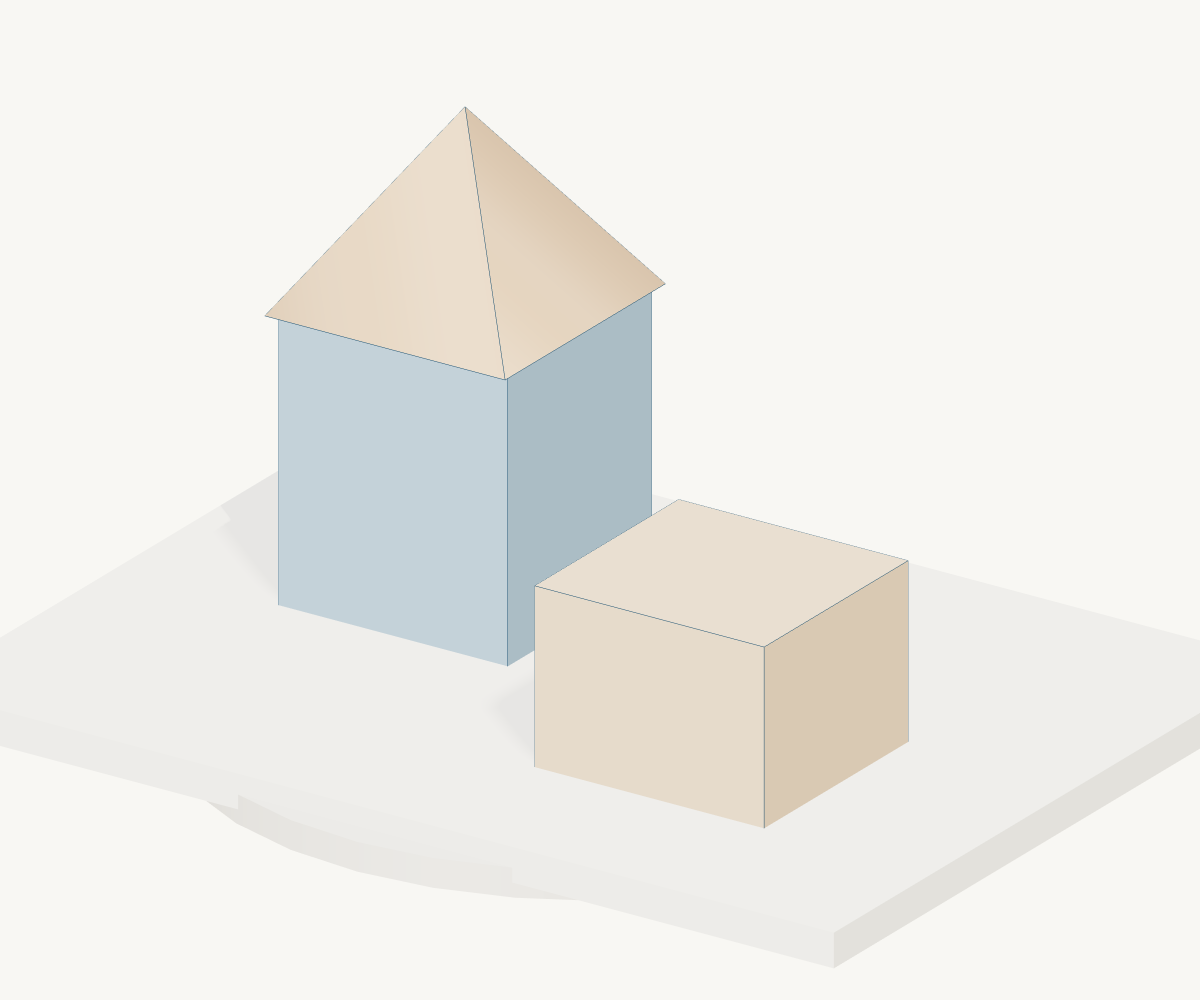
\includegraphics[width=1.30cm]{figures/img/main/three/renders/history_blocks.png}};
  \draw[arr] (-0.14,0.42) -- (0.15,0.42);
  % Orthographic basis for eye=(4,3.8,6), lookAt=(0,0.65,0), width=3.7.
  % Match the input's projection; the output omits the platform and shading.
  \begin{scope}[shift={(0.85,0.211)},
    x={(0.2923cm,-0.0780cm)},
    y={(0cm,0.3220cm)},
    z={(-0.1949cm,-0.1170cm)},
    visibleedge/.style={draw=steelblue31119180!85!black,line width=0.65pt},
    hiddenedge/.style={draw=black!35,line width=0.35pt,densely dashed}]
    \foreach \cx/\cy/\cz/\w/\h/\d in {-0.7/0.55/-0.3/0.85/1.0/0.8,0.65/0.36/0.30/0.85/0.62/0.80} {
      \begin{scope}[shift={(\cx,\cy,\cz)}]
        \coordinate (a) at ({-\w/2},{-\h/2},{-\d/2});
        \coordinate (b) at ({\w/2},{-\h/2},{-\d/2});
        \coordinate (c) at ({\w/2},{-\h/2},{\d/2});
        \coordinate (d) at ({-\w/2},{-\h/2},{\d/2});
        \coordinate (e) at ({-\w/2},{\h/2},{-\d/2});
        \coordinate (f) at ({\w/2},{\h/2},{-\d/2});
        \coordinate (g) at ({\w/2},{\h/2},{\d/2});
        \coordinate (h) at ({-\w/2},{\h/2},{\d/2});
        \draw[hiddenedge] (b) -- (a) -- (d) (a) -- (e);
        \draw[visibleedge] (b) -- (c) -- (d) -- (h) -- (e) -- (f) -- (g) -- (h)
          (b) -- (f) (c) -- (g);
        \foreach \v in {b,c,d,e,f,g,h}
          \fill[steelblue31119180!85!black] (\v) circle[radius=0.6pt];
      \end{scope}
    }
    % Four-sided roof: apex and base corners match the rendered pyramid.
    \coordinate (apex) at (-0.7,1.695,-0.3);
    \foreach \x/\z in {-1.145/-0.745,-0.255/-0.745,-0.255/0.145,-1.145/0.145} {
      \draw[visibleedge] (\x,1.045,\z) -- (apex);
    }
    \fill[steelblue31119180!85!black] (apex) circle[radius=0.7pt];
  \end{scope}
  \node[font=\scriptsize,align=center,text width=1.35cm] at (-0.87,-0.40) {image};
  \node[font=\scriptsize,align=center,text width=1.45cm] at (0.83,-0.40) {edges and\\vertices};
  \node[font=\scriptsize,draw=black!45,fill=white,rounded corners=1.5pt,
    align=center,text width=2.55cm,inner sep=4pt] at (0,-1.03) {3D structure};
\end{scope}
